Network-based approaches to cognitive neuroscience typically assume that mental
representations are encoded as distributed patterns of activation over large neural
populations, with different populations encoding different kinds of representational
structure and communicating this structure to other network components. Extensive research
over the past several years has focused on testing such hypotheses using data from
functional brain imaging techniques such as fMRI. The best-known approach in this vein has
been \emph{Representational Similarity Analysis} (RSA)~\cite{RSA}, which seeks to discover
brain regions whose activity encodes the known psychophysical similarities among some set
of stimuli. RSA is typically applied either to a specific brain region of interest (ROI)
or to many localized regions throughout the brain in process called  {\em searchlight
  analysis}~\cite{searchlight}.  For a given region, RSA computes the cosine distances
between the evoked responses for all stimulus pairs. The resulting neural dissimilarity
matrix is correlated with a target matrix of known psychophysical distances amongst the
stimuli. If these correlations are reliably non-zero, this suggests the corresponding
region may encode the similarity information.

A drawback of ROI and searchlight RSA is that these methods place strong assumptions on
the anatomical structure of the regions thought to encode the similarities of interest
(predefined ROIs or spherical clusters). In this paper we propose a new approach called
{\em Network RSA} that can discover arbitrarily structured brain networks (possibly widely
distributed and non-local) that encode similarity information. The key insight behind our
method is that RSA can be posed as a multi-task regression problem which, in conjunction
with sparsity regularization methods, can automatically detect networks of voxels that
appear to jointly encode similarity information.

Network RSA (NRSA) is summarized as follows (see Sections~\ref{wbrsa1}~and~\ref{wbrsa2}
for further details).  Consider a set of $n$ items and suppose we are given an $n \times
n$ similarity matrix $\bS$, where the $ij$-th element $\bS_{ij}$ is the known
psychophysical similarity \cite{similarity} between item $i$ and item $j$. For example,
these may come from human judgments of perceptual similarity between pairs of stimuli.
RSA is based on the hypothesis that there exists a set of voxels whose correlations across
stimuli encode the similarities in $\bS$, as depicted in Figure~\ref{fig.fitting}.

\begin{figure}[!h]
	\centering
	          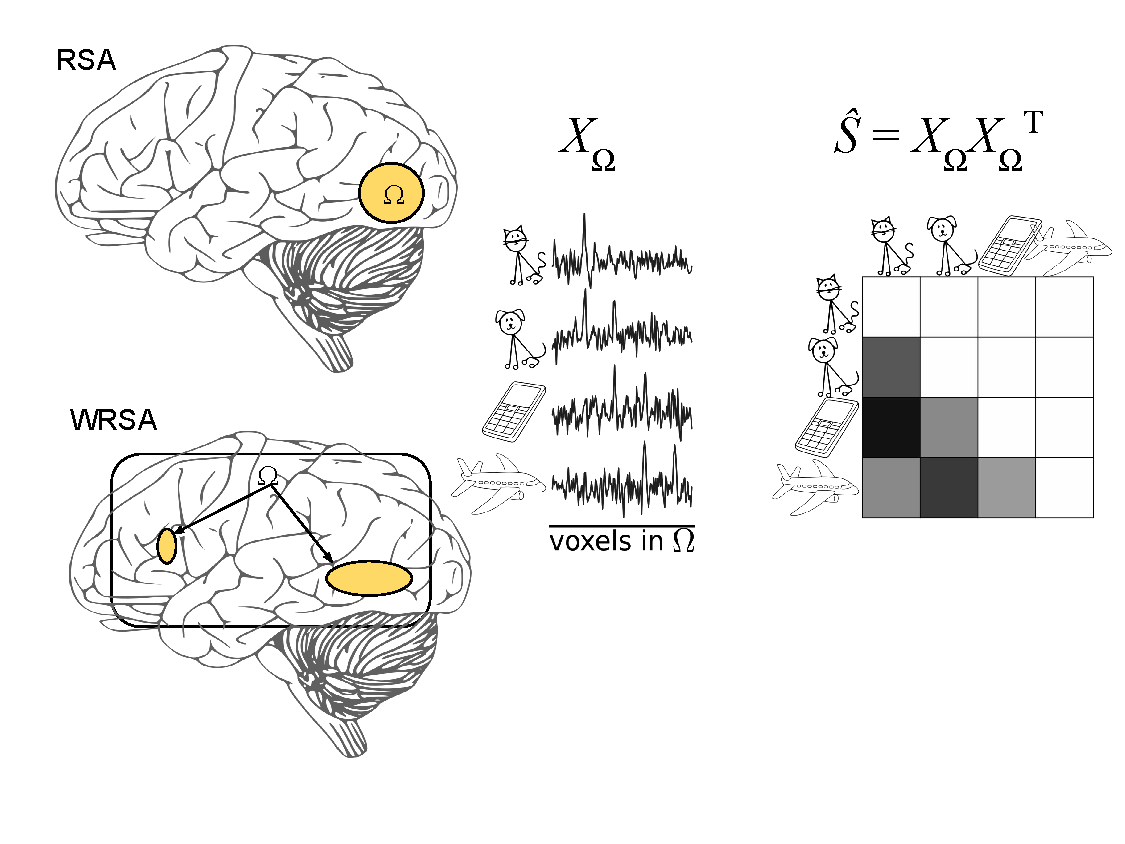
\includegraphics[width=0.5\textwidth]{WRSA.pdf}
	        
  \caption{Representational Similarity Analysis.  Traditional RSA methods consider only
    localized brain networks, such as specific regions of interest or spherical clusters
    of the cortex (upper left)~\cite{RSA,searchlight}.  We propose a new {\em Network} RSA
    (NRSA) method that can potentially identify non-local brain networks that encode
    similarity information (lower left).  Within a set of voxels $\Omega$ (localized or
    non-local), the correlations between the activation patterns resulting from different
    stimuli approximate (perceptual) similarities between the stimuli.  } \label{Fig:WRSA}
	\label{fig.fitting}
\end{figure}

Let $\bX \in \R^{n\times p}$ denote a matrix of voxel activations.
Each row corresponds to activations in all $p$ voxels in response to a specific stimulus,
and each column corresponds to the activations in specific voxel to the $n$ different
stimuli.  Our generalized notion of RSA, which encompasses conventional ROI \cite{RSA} and
searchlight \cite{searchlight} approaches, involves finding a sparse symmetric positive
semi-definite matrix  $\bW\in \R^{p\times p}$ such that

$$\bS \ \approx \bX \bW \bX^T \ .$$

By sparse we mean that at most $k<p$ rows/columns of $\bW$ are nonzero. The locations of
the nonzero elements indicate which voxels are included in the similarity-encoding brain
network, and the weights in $\bW$ indicate the strength of the edges in the network.  For
instance, consider the $n\times 1$ activation vectors of two voxels $\bx_k$ and
$\bx_{\ell}$ (i.e., the $k$th and $\ell$th columns of $\bX$).  It is easy to show that the
contribution of these two voxels to the similarity representation is given by $ W_{k,\ell}
\, \bx_k \bx_{\ell}^T + W_{\ell,k} \, \bx_\ell \bx_{k}^T$.  If $W_{k,\ell}=W_{\ell,k}\neq
0$, then the correlations between the two voxels contribute to the approximation of the
similarity matrix $\bS$. The complete similarity representation can be expressed as
$$\bS \ \approx \ \bX\bW\bX^T \ = \ \sum_{k,\ell=1}^p W_{k,\ell} \, \bx_k \bx_{\ell}^T  \ .$$

The approximation problem can be posed as the least squares optimization

$$\min_{\bW} \|\bS-\bX\bW\bX^T\|_F^2 \ , $$

where the objective is the Frobenius norm of the difference between the similarity matrix
$\bS$ and its approximation in terms of voxel activations. Since $\bS$ is a positive
semi-definite matrix, there exists a matrix $\bY$ which satisfies $\bS=\bY\bY^T$ (e.g.,
obtained via eigendecomposition or Cholesky decomposition).  Thus, we may instead consider
the optimization

$$\min_{\bB} \|\bY-\bX\bB\|_F^2 \ . $$

For any coefficient matrix $\bB$ the corresponding weight matrix is given by $\bW =
\bB\bB^T$. Both optimizations are convex, but we will work with the latter since it tends
to be easier to solve and also allows us to easily incorporate constraints or
regularizers.

The weight matrix $\bW$ and the coefficient matrix $\bB$ are often expected to exhibit
sparsity and low-rank structure. Indeed, the hypothesis underlying RSA is that a small
subset of the brain encodes the similarity representations, hence the sparsity.
Similarity matrices are often low-rank because of clustering or other relationships
between the items under consideration. For example, in our experimental application
described later in the paper, we find that a rank $r=3$ approximation is quite accurate.
Since the voxel activations represent noisy measurements of brain regions, we also expect
$\bW$ and $\bB$ to be low-rank to encourage clustering in the selected voxels.  To account
for this, the optimization above can be modified to obtain sparse and low-rank solutions,
as described next.



\section{Learning Similarity Encodings via Group Lasso}

Consider the group lasso optimization
\begin{equation}\label{eqn.grouplasso}
 \min_{\bB\in \R^{p\times r}} \|\bY-\bX\bB\|_F^2 \ + \ \lambda \|\bB\|_{1,2}  \ .
 \end{equation}
Note that the optimization variable $\bB$ is a $p\times r$ matrix, which guarantees a rank
$r$ (or less) solution, and thus similarity representation $\bX\bB\bB^T\bX^T$ will be rank
$r$ at most, which is a simple way to enforce the low-rank constraint.  The parameter
$\lambda>0$ is an adjustable weight on the sparsity-promoting regularizer
$\|\bB\|_{1,2}$, which is defined as follows. The rows of $\bB$ are denoted by
$\bbeta_{i\a}$, $i=1,\dots,p$, and the norm
$\|\bB\|_{1,2} \ = \ \sum_{i=1}^n \|\bbeta_{i\a}\|_2$. This encourages solutions with only
a few nonzero rows in $\bB$ \cite{obo11,lounici,vandegeer}.

The main technical innovation in this paper is a new approach to the group lasso that is
designed to cope with strongly correlated covariates (\ie cases in which certain columns
of $\bX$ may be close to, or even exactly, collinear).  This is a concern in fMRI, since
certain voxels may have very correlated activation patterns. This problem is illustrated
in Figure~\ref{Fig:sim}, where we simulate a situation where columns $5$ and $7$ of the
data matrix $\bX$ are highly correlated. Group lasso selects one of the corresponding rows
in $\bB$ (row $5$), whereas GrOWL correctly selects both rows $5$ and $7$. 

In the standard (single-task) regression problem, this issue has been tackled using many
techniques, including the elastic net \cite{EN}, OSCAR \cite{oscar} and OWL \cite{owl},
and others.  We propose a generalization of the recently proposed Ordered Weighted
$\ell_1$ (OWL) approach to the multi-task setting, and thus call our new approach Group
OWL (GrOWL). We show that GrOWL shares many of the desirable features of the OWL method,
namely it automatically clusters and averages regression coefficients associated with
strongly correlated columns of $\bX$.  This has two desirable effects, in terms of both
model selection and prediction.  First, GrOWL can select all of the relevant voxels in
$\bX$, unlike standard group lasso which may not select relevant voxels if they happen to
be strongly correlated with others.  Second, GrOWL encourages the coefficients associated
with strongly correlated voxels to be near or exactly equal.   In effect, this averages
strongly correlated voxels which can help to denoise activation patterns and improve
predictions.


\begin{figure}[!t]
    \centering
    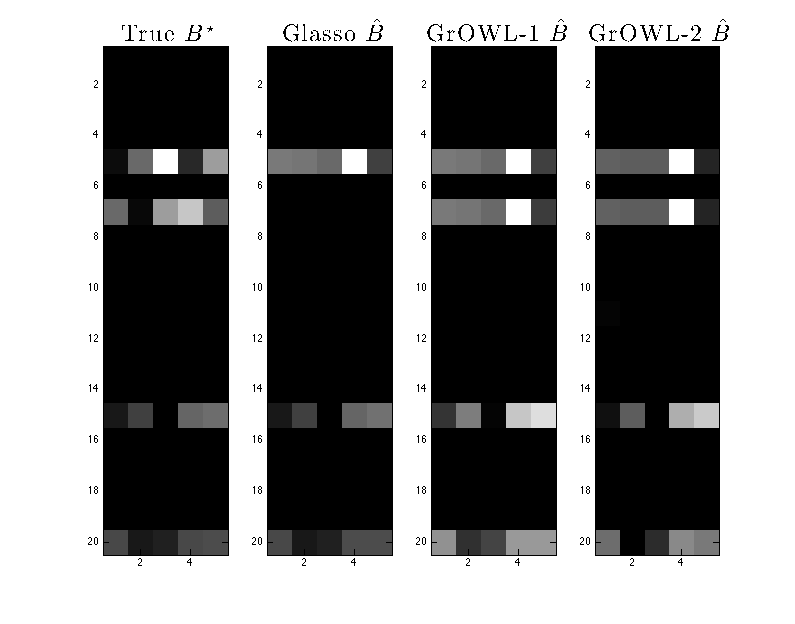
\includegraphics[width=0.6\linewidth]{sim3.png}
    \qquad
   \caption{A comparison of group lasso and grOWL optimization solutions with correlated columns in $\bX$ showing that GrOWL selects relevant features (row 5 and 7) even if they happen to be strongly correlated and automatically cluster them by setting the corresponding coefficient rows to be equal (or nearly equal).}
    \label{Fig:sim}
  \end{figure}
